\documentclass{tufte-handout}
\usepackage{pgfplots}
\usepackage[dvipsnames]{xcolor}
\usepackage{ulem}
\usepackage{subcaption}
\usepackage{amssymb, amsmath, pgfplots, tabularx, siunitx}
\usepackage{algorithm}
\usepackage{makecell}
\usepackage{amsfonts}
\pgfplotsset{compat = newest}

\usepackage{tikz}
\usetikzlibrary{shadings}
\usetikzlibrary{calc,arrows.meta}
\usetikzlibrary{shapes.misc}
\usepackage[most]{tcolorbox}
\usepgfplotslibrary{colormaps,patchplots}

\definecolor{wp-bg}{HTML}{FDF6EF}
\definecolor{wp-text}{HTML}{2D1B0E}
\definecolor{wp-primary}{HTML}{C24A3A}
\definecolor{wp-accent}{HTML}{D4952E}
\definecolor{wp-light}{HTML}{F0DECA}
\definecolor{wp-muted}{HTML}{C4A88A}
\definecolor{wp-dark}{HTML}{1A0F07}
\definecolor{wp-code}{HTML}{FDF2E4}

\pagecolor{wp-bg}
\color{wp-text}

\hypersetup{colorlinks=true,linkcolor=wp-primary,urlcolor=wp-accent}

\tikzset{basic/.style={draw,text width=1em,text badly centered}}
\tikzset{input/.style={basic,circle}}
\tikzset{weights/.style={basic,rectangle}}
\tikzset{functions/.style={basic,circle}}

\title{Machine Learning Notes \\ Preliminary Introduction to Deep Learning}
\author{Vitor Negromonte Cabral de Oliveira}

\date{December 2024}

\begin{document}

\maketitle
\begin{abstract}
    This notebook serves as a comprehensive repository for my Machine Learning studies, with a primary focus on Deep Learning. Key topics covered include:
    \begin{itemize}
        \item Artificial Neural Networks (ANNs) – Fundamentals and architectures with mathematical explaination.
    \end{itemize}
\end{abstract}

\newpage
\hypersetup{linkcolor=wp-text}
\tableofcontents
\hypersetup{linkcolor=wp-primary}
\newpage
\section{Introdução à Neurônios Artificiais}

\subsection{Perceptron}

Quase toda rede neural artificial moderna — desde classificadores simples até arquiteturas complexas de deep learning, tem suas origens em uma unidade computacional simples chamada perceptron \sidenote{Embora a maioria das redes neurais dependa de unidades semelhantes ao perceptron, existem paradigmas alternativos, como o aprendizado Hebbiano (inspirado na plasticidade sináptica) e a recentemente revivida Rede Kolmogorov-Arnold (KAN), que dispensa completamente as estruturas tradicionais de neurônios.}.

Desenvolvido por Frank Rosenblatt em 1947, inspirado no trabalho de McCulloch e Pitts em 1943. O perceptron se baseia na interpretação matemática do funcionamento de neurônios biológicos.

Em sua essência, um perceptron é um mecanismo de decisão binário. Ele recebe um conjunto de valores reais, pondera sobre sua "importância"\sidenote{} e faz uma escolha baseada em um limiar de decisão. Imagine o perceptron como um pequeno porteiro: ele avalia as evidências (entradas), aplica seus próprios vieses e preferências (pesos) e entrega um veredito — ou 1 (“sim”) ou 0 (“não”)\sidenote{Original, o valores eram 1 e -1, para "sim" e "não". Decidi por deixar na interpretação mais comum de 0 e 1.}


\paragraph{Fundamentação matemática de Perceptrons}

Dado um conjunto de entradas $\mathbf{X}$ com valores $x_1, x_2, ..., x_n$ a saída do perceptron ($\mathbf{Y}$) é calculada em dois passos:
\begin{enumerate}
    \item Soma ponderada: Calcula a combinação linear das entradas, ajustadas pelos pesos $w_i$ e o viés $b$ (que funciona para ajustar as fronteiras de decisão):
    \begin{equation}
        z = w_0 + \sum_{i=1}^{n}w_ix_i
    \end{equation}
    \item Thresholding: Aplica uma função degrau para produzir a saída final:
    \begin{equation} \label{perceptron}
    o(x_1, \dots, x_n) =
    \begin{cases}
    1 & \text{se } w_0 + \sum_{i=1}^n w_i x_i > 0 \quad \text{(ativação)}, \\ 0 & \text{otherwise.}
    \end{cases}
    \end{equation}
\end{enumerate}

Cada peso \( w_i \), é uma constante real também chamada de \textit{parâmetro}, que determina a contribuição da entrada $x_i$ para a saída do perceptron. O viés funciona como um limite ajustável: a soma ponderada $\sum_{i=1}^n w_i x_i$ precisa exceder $-b$ para uma saída de ativação $+1$. Para simplificar a notação, adicionamos uma entrada constante $x_0 = 1$, permitindo que a condição de ativação seja escrita de maneira compactada como $\sum_{i=0}^n w_i x_i > 0$ ou, na forma vetorial, $\mathbf{w} \cdot \mathbf{x} > 0$.

O Perceptron pode ser usado para representar muitas funções booleanas — na verdade, ele pode representar todas as funções booleanas primitivas (AND, OR, NAND e NOR). No entanto, algumas funções booleanas não podem ser representadas por um único perceptron, como é o caso da função XOR, cujo valor é 1 quando e somente quando $x_1 \neq x_2$. Essa limitação de uma única unidade de perceptron em não conseguir representar a função XOR marcou o início do que ficou conhecido como o primeiro inverno da Inteligência Computacional.


\paragraph{Interpretação Geométrica do Perceptron}

O mecanismo de decisão do perceptron admite uma interpretação geométrica. Considere um perceptron com $n$ entradas: seu vetor de pesos $\mathbf{w} = (w_0, w_1, ..., w_n)$ e o vetor de entradas $\mathbf{x} = (1, x_1, ..., x_n)$ definem um hiperplano no espaço $\mathbb{R}^{n+1}$:


\begin{equation}
    \mathbf{w} \cdot \mathbf{x} = w_0 + \sum_{i=1}^n w_i x_i = 0
\end{equation}
Essa \textit{fronteira de decisão} divide o espaço de entrada em duas regiões distintas:

\begin{itemize}
\item $\mathbf{w} \cdot \mathbf{x} > 0$ corresponde à saída $+1$ (classe positiva)
\item $\mathbf{w} \cdot \mathbf{x} < 0$ corresponde à saída $-1$ (classe negativa)
\end{itemize}

No caso especial de entradas bidimensionais ($x_1, x_2$), isso se reduz a uma reta em $\mathbb{R}^2$:

\begin{equation}
w_0 + w_1x_1 + w_2x_2 = 0
\end{equation}

\begin{figure}[h]
\centering
    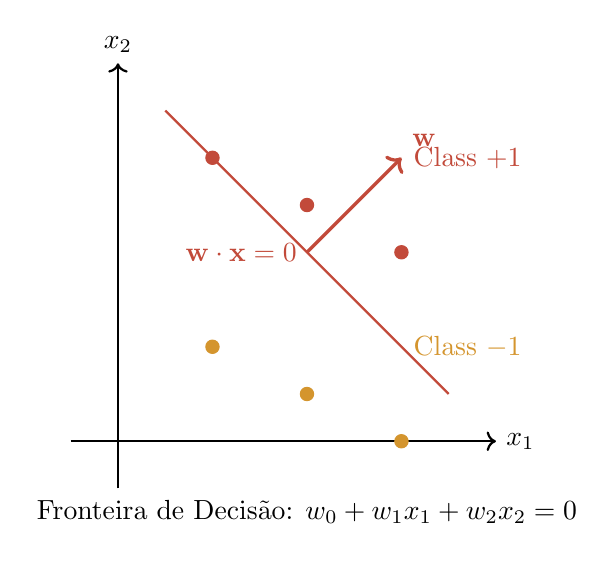
\begin{tikzpicture}[scale=1.2]

    % Axes
    \draw[->, thick] (-0.5,0) -- (4,0) node[right]{$x_1$};
    \draw[->, thick] (0,-0.5) -- (0,4) node[above]{$x_2$};

    % Decision boundary (w0 + w1x1 + w2x2 = 0)
    \draw[wp-primary, thick] (0.5,3.5) -- (3.5,0.5) node[midway, left]{$\mathbf{w}\cdot\mathbf{x}=0$};

    % Weight vector (normal to boundary)
    \draw[->, wp-primary, very thick] (2,2) -- (3,3) node[above right]{$\mathbf{w}$};

    % Positive examples (output +1)
    \filldraw[wp-primary] (1,3) circle (2pt) node[above right]{};
    \filldraw[wp-primary] (2,2.5) circle (2pt) node[above right]{};
    \filldraw[wp-primary] (3,2) circle (2pt) node[above right]{};

    % Negative examples (output -1)
    \filldraw[wp-accent] (1,1) circle (2pt) node[below left]{};
    \filldraw[wp-accent] (2,0.5) circle (2pt) node[below left]{};
    \filldraw[wp-accent] (3,0) circle (2pt) node[below left]{};

    % Class labels
    \node[wp-primary] at (3.7,3) {Class $+1$};
    \node[wp-accent] at (3.7,1) {Class $-1$};

    % Equation
    \node at (2,-0.75) {Fronteira de Decisão: $w_0 + w_1x_1 + w_2x_2 = 0$};

\end{tikzpicture}
\end{figure}


O termo de viés $w_0$ determina o deslocamento em relação à origem, enquanto a razão $w_1/w_2$ define a inclinação. O vetor de pesos $\mathbf{w}$ é sempre \textit{normal} (perpendicular) à fronteira de decisão, apontando na direção da região positiva.

Essa perspectiva geométrica revela a limitação fundamental do perceptron: ele só é capaz de aprender funções linearmente separáveis. O clássico problema do XOR exemplifica bem essa restrição — nenhuma linha pode separar $(0,1)$ e $(1,0)$ de $(0,0)$ e $(1,1)$ em $\mathbb{R}^2$. Essa limitação motivou o desenvolvimento dos perceptrons multicamadas (MLPs), capazes de construir fronteiras de decisão não lineares por meio da composição de múltiplos hiperplanos.

\paragraph{The XOR Problem}

O “Problema do XOR” é um problema clássico em Inteligência Computacional, proposto inicialmente por Marvin Minsky em seu livro Perceptrons (1969). Trata-se do problema de usar um Perceptron para prever a saída de uma porta lógica XOR dadas duas entradas binárias. Uma função XOR deve retornar verdadeiro somente se as duas entradas forem diferentes, e falso se forem iguais.

A estrutura de uma unidade de perceptron é limitada a separar pontos de dados com uma única linha, e como as entradas do XOR não são linearmente separáveis, o perceptron simples falha nessa tarefa. Esse problema pode ser resolvido adicionando uma camada extra de neurônios à rede, chamada camada oculta. Essa arquitetura é conhecida como Perceptron Multicamadas (discutida na próxima seção).

\begin{figure}[h]
    \centering
    % Subfigure for the table
    \begin{subfigure}{0.45\textwidth}
        \centering
        \begin{tabular}{c|c|c}
            Input 1 & Input 2 & Output \\
            \hline
            0 & 0 & 0 \\
            \hline
            1 & 0 & 1 \\
            \hline
            0 & 1 & 1 \\
            \hline
            1 & 1 & 0 \\
        \end{tabular}
        \caption{XOR truth table}
        \label{tab:xor}
    \end{subfigure}
    % Subfigure for the plot
    \begin{subfigure}{0.45\textwidth}
        \centering
        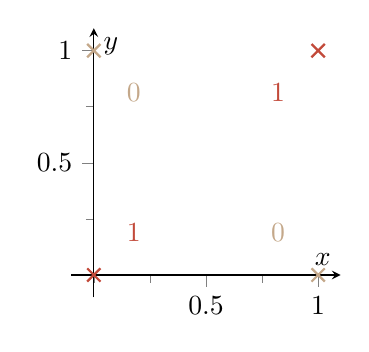
\begin{tikzpicture}
            \tikzstyle{point}=[thick,draw=wp-text,cross out,inner sep=0pt,minimum width=4pt,minimum height=4pt]
            \begin{axis}[
                legend pos=south west,
                axis x line=middle,
                axis y line=middle,
                grid=none,
                width=5cm,
                height=5cm,
                grid style={dashed, wp-muted!30},
                xmin=0,    % start the diagram at this x-coordinate
                xmax=1,    % end   the diagram at this x-coordinate
                ymin=0,    % start the diagram at this y-coordinate
                ymax=1,    % end   the diagram at this y-coordinate
                xlabel=$x$,
                ylabel=$y$,
                tick align=outside,
                minor tick num=-3,
                enlargelimits=true]
              \node[point,label={[label distance=0.3cm,text=wp-muted]135:$0$},wp-muted] at (axis cs:1,0) {};
              \node[point,label={[label distance=0.3cm,text=wp-muted]-45:$0$},wp-muted] at (axis cs:0,1) {};
              \node[point,label={[label distance=0.3cm,text=wp-primary]45:$1$},wp-primary] at (axis cs:0,0) {};
              \node[point,label={[label distance=0.3cm,text=wp-primary]-135:$1$},wp-primary] at (axis cs:1,1) {};
            \end{axis}
        \end{tikzpicture}
        \caption{XOR visualization}
        \label{fig:xor_plot}
    \end{subfigure}
    % Combined caption
    \caption{XOR operation represented as a truth table (a) and a visualization (b). The plot shows the XOR output for different inputs, where $0$s are marked in \textcolor{wp-muted}{wp-muted} and $1$s are marked in \textcolor{wp-primary}{wp-primary}.}
    \label{fig:xor_combined}
\end{figure}
    

\subsection{Gradiente Descendente e Gradiente Descendente Estocástico}
\paragraph{Regra de Treinamento do Perceptron}
Uma maneira de aprender um vetor de pesos adequado é começar com pesos aleatórios e, então, aplicar o perceptron iterativamente a cada exemplo de treinamento, modificando seus pesos sempre que ele classifica um exemplo incorretamente. Esse processo é repetido, percorrendo os exemplos de treinamento quantas vezes for necessário, até que o perceptron classifique corretamente todos os exemplos.

Os pesos são modificados a cada etapa de acordo com a regra de treinamento do perceptron, que ajusta o peso $w_i$ associado à entrada $x_i$ da seguinte forma:

\begin{equation}
w_i \leftarrow w_i + \Delta w_i
\end{equation}

onde

\begin{equation}
\Delta w_i = \eta (t - o)x_i
\end{equation}

Aqui, $t$ representa a saída desejada (alvo) para o exemplo de treinamento atual, $o$ é a saída gerada pelo perceptron, e $\eta$ é uma constante positiva chamada taxa de aprendizado (learning rate).
A função da taxa de aprendizado é moderar o quanto os pesos são ajustados em cada passo. Geralmente, ela é definida com um valor entre 0 e 1, e às vezes é reduzida gradualmente à medida que o número de iterações de ajuste de pesos aumenta.

\paragraph{Delta Rule}
Embora a regra do perceptron encontre um vetor de pesos bem-sucedido quando os exemplos de treinamento são linearmente separáveis, ela pode não convergir se os exemplos não forem linearmente separáveis. Uma segunda regra de treinamento, chamada regra delta, foi desenvolvida para superar esse problema.

A ideia central da regra delta é usar o gradiente descendente para buscar, no espaço de hipóteses dos possíveis vetores de pesos, aqueles que melhor se ajustam aos exemplos de treinamento. Essa regra serve de base para o algoritmo de retropropagação (Backpropagation).

A regra delta é melhor compreendida considerando o treinamento de um perceptron sem limiar (unthresholded perceptron), isto é, uma unidade linear cuja saída $o$ é dada por:

\begin{equation}
o(\Vec{x}) = \Vec{w} \cdot \Vec{x}
\end{equation}

Assim, uma unidade linear corresponde à primeira etapa de um perceptron, sem a função de limiar.
Para derivar uma regra de aprendizado de pesos para unidades lineares, começamos definindo uma medida de erro de treinamento de uma hipótese em relação aos exemplos de treinamento. Embora existam várias maneiras de definir o erro, uma medida comum e particularmente conveniente é:

\begin{equation} \label{eq:7}
E(\Vec{w}) = \frac{1}{2}\sum_{d\in D} (t_d - o_d)^2
\end{equation}

onde $D$ é o conjunto de exemplos de treinamento, $t_d$ é a saída desejada (alvo) para o exemplo $d$, e $o_d$ é a saída da unidade linear para esse exemplo.

\paragraph{Gradient Descent}

Para compreender melhor o Gradiente Descendente, é útil visualizar todo o espaço de hipóteses dos possíveis vetores de pesos e seus respectivos valores de erro $E$ (Figura \ref{fig:GD}).
O processo de busca do gradiente descendente determina um vetor de pesos que minimiza $E$, começando com um vetor de pesos inicial arbitrário e modificando-o repetidamente em pequenos passos.
A cada passo, o vetor de pesos é ajustado na direção que produz a maior descida ao longo da superfície de erro, conforme ilustrado na Figura \ref{fig:GD}.

\begin{figure}
\centering
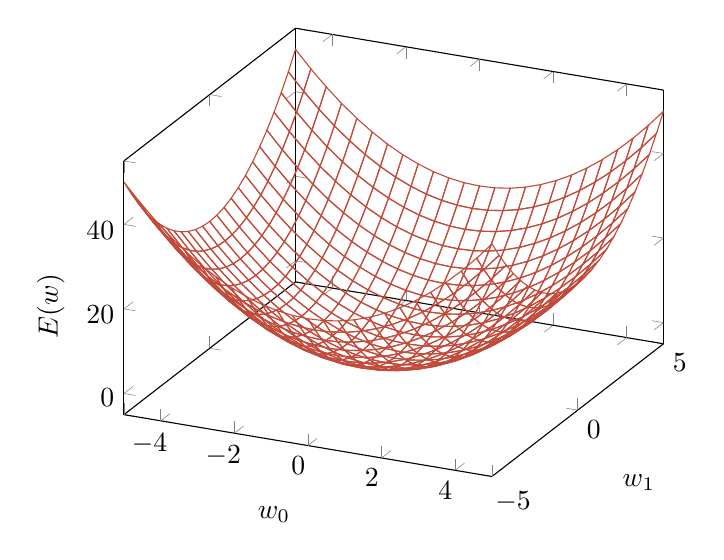
\begin{tikzpicture}  
    \begin{axis}[
        xlabel = {$w_0$},
        ylabel = {$w_1$},
        zlabel = {$E(w)$},
    ]
    
    	\addplot3[
        mesh,
        draw = wp-primary!100!white
        ] {x^2 + y^2};
    
    \end{axis}
\end{tikzpicture}
\caption{Generic representation of a hypothesis space}
\label{fig:GD}
\end{figure}
Com base nisso, podemos calcular a direção de maior descida ao longo da superfície de erro ($E$), computando a derivada de $E$ em relação a cada componente do vetor $\Vec{w}$.
Essa derivada vetorial é chamada de gradiente de $E$ em relação a $\Vec{w}$, e é escrita como $\nabla E(\Vec{w})$:

\begin{equation}
\nabla E(\Vec{w}) \equiv
\left[ \frac{\partial E}{\partial w_0}, \frac{\partial E}{\partial w_1}, ..., \frac{\partial E}{\partial w_n} \right]
\end{equation}

$\nabla E(\Vec{w})$ é, portanto, um vetor cujos componentes são as derivadas parciais de $E$ em relação a cada $w_i$. Interpretado no espaço dos pesos, o gradiente indica a direção que produz o maior aumento de $E$.

Como queremos minimizar $E$, o vetor de pesos é atualizado na direção oposta ao gradiente, conforme a seguinte regra de aprendizado:

\begin{equation}
\Vec{w} \leftarrow \Vec{w} + \Delta \Vec{w}
\end{equation}

onde

\begin{equation}
\Delta \Vec{w} = - \eta \nabla E(\Vec{w})
\end{equation}

O sinal negativo está presente porque desejamos mover o vetor de pesos na direção que reduz $E$. Essa regra de treinamento também pode ser escrita em sua forma componente:

\begin{equation}
w_i \leftarrow w_i + \Delta w_i
\end{equation}

onde

\begin{equation}
\Delta w_i = -\eta\frac{\partial E}{\partial w_i}
\end{equation}

Para calcular eficientemente o gradiente em cada passo, precisamos obter as derivadas $\frac{\partial E}{\partial w_i}$, diferenciando $E$ da Equação \ref{eq:7}:

\begin{equation}
    \begin{split}
        \frac{\partial E}{\partial w_i} &= \frac{\partial}{\partial w_i} \frac{1}{2} \sum_{d \in D} (t_d - o_d)^2 \\
        &= \frac{1}{2} \sum_{d \in D} \frac{\partial}{\partial w_i} (t_d - o_d)^2 \\
        &= \frac{1}{2} \sum_{d \in D} 2 (t_d - o_d) \frac{\partial}{\partial w_i} (t_d - o_d) \\
        &= \sum_{d \in D} (t_d - o_d) \frac{\partial}{\partial w_i} (t_d - \vec{w} \cdot \vec{x}_d) \\
        &= \sum_{d \in D} (t_d - o_d)(-x_{id})
    \end{split}
\end{equation}

onde $x_{id}$ denota o componente de saída individual $x_i$ para o exemplo de treinamento $d$.
Com tudo isso, agora temos uma equação que expressa $\frac{\partial E}{\partial w_i}$ em termos das entradas da unidade linear $x_{id}$, das saídas $o_d$ e dos valores-alvo $t_d$ associados aos exemplos de treinamento. Assim, obtemos:

\begin{equation}
\Delta w_i = \eta \sum_{d \in D} (t_d - o_d)x_{id}
\end{equation}

Devido à sua complexidade computacional, normalmente não utilizamos o Gradiente Descendente (GD) diretamente.
A necessidade de usar o conjunto inteiro de dados em cada iteração durante o treinamento torna o GD computacionalmente caro.
Por isso, utiliza-se uma aproximação estocástica do gradiente descendente, geralmente chamada de Gradiente Descendente Estocástico (SGD).

No SGD, em vez de usar todo o conjunto de dados a cada iteração, apenas um subconjunto aleatório é selecionado para calcular o gradiente e atualizar os parâmetros do modelo.
Essa seleção aleatória introduz aleatoriedade no processo de otimização (o termo estocástico se refere a algo descrito por uma distribuição de probabilidade aleatória).
Matematicamente, isso pode ser descrito como:

\begin{equation}
w_i := w_i - \eta \nabla Q_i (w)
\end{equation}

A aleatoriedade da técnica também pode introduzir ruído no gradiente, resultando em algumas variações bruscas durante o processo de otimização.

\subsection{Multilayer Perceptron and Backpropagation}
Para lidar com as limitações de um único neurônio artificial — que só pode representar fronteiras de decisão lineares — exploramos o conceito de uma rede multicamadas.
Nessa abordagem, várias camadas totalmente conectadas são empilhadas umas sobre as outras, permitindo que o modelo aprenda e represente superfícies de decisão mais complexas e não lineares.

Para fins didáticos, chamaremos a rede anterior (perceptron) de Rede Neural Rasa (Shallow Neural Network). Esse termo é usado porque, em uma única camada de neurônios, a única forma de aumentar a capacidade da rede é adicionar mais neurônios verticalmente, ou seja, na mesma camada.
Neste capítulo, exploraremos a evolução desses conceitos — das Redes Rasas às Redes Neurais Profundas (Deep Neural Networks) — e seus impactos na área.

A maneira mais simples de tornar uma rede neural mais profunda é compor várias redes rasas. Basicamente, a saída de uma unidade serve como entrada para a próxima unidade.

À primeira vista, precisamos decidir que tipo de unidade usaremos como base para construir redes multicamadas. Inicialmente, pode parecer natural escolher as unidades lineares discutidas anteriormente, já que já derivamos uma regra de aprendizado por gradiente descendente para elas.
Contudo, múltiplas camadas de unidades lineares em cascata ainda produzem apenas funções lineares.
O que precisamos é de uma unidade cuja saída seja uma função não linear e diferenciável de suas entradas — como uma sigmoide, tangente hiperbólica (tanh) ou ReLU —, qualquer função que atenda a esses requisitos pode ser utilizada.


\paragraph{Backpropagation Algorithm }
O algoritmo de Backpropagation (BP) aprende os pesos de uma rede multicamadas, considerando uma rede com um conjunto fixo de unidades e interconexões.
Ele utiliza o gradiente descendente para minimizar o erro quadrático entre as saídas da rede e os valores-alvo correspondentes.

Como agora consideramos redes com múltiplas unidades de saída (em vez de apenas uma, como antes), redefinimos a função de erro $E$ para somar os erros de todas as unidades de saída da rede:

\begin{equation}
E(\Vec{w}) \equiv \frac{1}{2} \sum_{d \in D} \sum_{k \in \text{outputs}} (t_{kd} - o_{kd})^2
\end{equation}

onde outputs é o conjunto de unidades de saída da rede, e $t_{kd}$ e $o_{kd}$ são, respectivamente, os valores-alvo e as saídas associadas à $k$-ésima unidade de saída para o exemplo de treinamento $d$.

O problema de aprendizado enfrentado pela Retropropagação consiste em buscar, dentro de um grande espaço de hipóteses, definido por todos os possíveis valores de pesos das unidades da rede, aqueles que minimizam o erro $E$.
Assim como no caso de uma única unidade, o gradiente descendente é usado para tentar encontrar a hipótese que minimize $E$.

Uma diferença importante no caso das redes multicamadas é que a superfície de erro pode possuir múltiplos mínimos locais, ao contrário da superfície parabólica com mínimo único observada no caso simples.
Isso significa que o gradiente descendente só é garantido a convergir para algum mínimo local, não necessariamente para o mínimo global.

O algoritmo segue os seguintes passos:

\begin{itemize}
\item Cada exemplo de treinamento é um par $\langle \Vec{x}, \Vec{t} \rangle$, onde $\Vec{x}$ é o vetor de entradas da rede e $\Vec{t}$ é o vetor de saídas-alvo.
\item $\eta$ é a taxa de aprendizado. $n_{in}$ é o número de entradas, $n_{hidden}$ o número de unidades na camada oculta, e $n_{out}$ o número de unidades de saída.
\item A entrada da unidade $i$ na unidade $j$ é denotada por $x_{ij}$, e o peso correspondente é $w_{ij}$.
\end{itemize}

The Backpropagation algorithm involves two phases for each training example:

\paragraph{Forward Pass:} 
\begin{enumerate}
    \item Initialize the network by assigning random small values to all weights $w_{ij}$.
    \item Present the input vector $\Vec{x}$ to the input layer.
    \item Propagate the activations forward through the network using the activation function $o_j = f\big( \sum_i w_{ij} x_{ij} \big)$, where $f$ is a differentiable activation function (e.g., sigmoid or ReLU).
\end{enumerate}

\paragraph{Backward Pass (Error Computation and Weight Update):}
\begin{enumerate}
    \item Compute the error for the output layer: $\delta_k = (t_k - o_k)f'(o_k)$, where $f'(o_k)$ is the derivative of the activation function.
    \item Compute the error for the hidden layer units: $\delta_j = f'(o_j) \sum_k w_{jk} \delta_k$.
    \item Update the weights for each layer using the gradient descent rule:
    \begin{equation}
        w_{ij} \leftarrow w_{ij} + \eta \cdot \delta_j \cdot o_i
    \end{equation}
    where $\eta$ is the learning rate and $o_i$ is the activation of the input to unit $j$.
\end{enumerate}

\paragraph{Repeat:}
Repeat the above steps for each training example until convergence or until a predefined number of iterations is reached. Convergence is achieved when the total error $E(\Vec{w})$ is sufficiently small or no longer decreases significantly.

This process allows the network to adjust its weights iteratively to minimize the error and improve its performance on the training data. While convergence to a global minimum cannot be guaranteed due to the potential for local minima, this algorithm provides a practical and effective approach for training multilayer neural networks.

\begin{algorithm}[h]
    \caption{Backpropagation Algorithm}
        \textbf{Input:} Training examples $\langle \Vec{x}, \Vec{t} \rangle$, where $\Vec{x}$ is the input vector and $\Vec{t}$ is the target vector. \\
        \textbf{Output:} Trained weights $w_{ij}$ minimizing the error function. \\
        \textbf{Initialize:} Randomly set all weights $w_{ij}$ to small values. Set the learning rate $\eta > 0$. \\
        
        \textbf{Forward Pass} \\
        1. Present the input vector $\Vec{x}$ to the network. \\
        2. For each neuron $j$ in hidden and output layers, compute: \\
        \begin{equation*}
            o_j = f\left(\sum_i w_{ij} x_{ij}\right)
        \end{equation*}
        where $f(\cdot)$ is a differentiable activation function (e.g., sigmoid, ReLU). \\
        
        \textbf{Backward Pass} \\
        1. Compute the error signal $\delta_k$ for each output unit $k$: \\
        \begin{equation*}
            \delta_k = (t_k - o_k) f'(o_k)
        \end{equation*}
        2. Compute the error signal $\delta_j$ for each hidden unit $j$: \\
        \begin{equation*}
            \delta_j = f'(o_j) \sum_k w_{jk} \delta_k
        \end{equation*}
        3. Update the weights $w_{ij}$ for each connection: \\
        \begin{equation*}
            w_{ij} \leftarrow w_{ij} + \eta \cdot \delta_j \cdot o_i
        \end{equation*}

        Repeat
        Perform the \textit{Forward Pass} and \textit{Backward Pass} for all training examples. \\
        Until Convergence is achieved (e.g., total error $E(\Vec{w})$ becomes sufficiently small or stops decreasing).
\end{algorithm}

\subsection{Universal Approximation Theorem}
\begin{figure}[h]
\centering
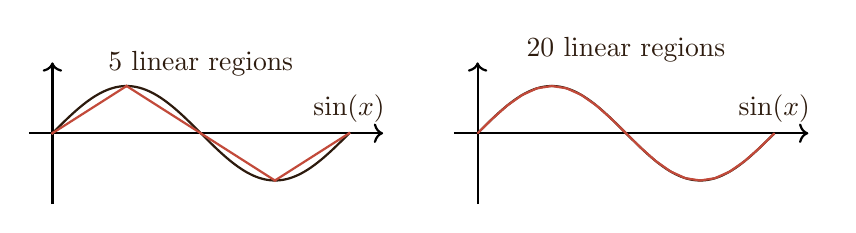
\begin{tikzpicture}[scale=0.6, thick]

    % First plot: 5 linear regions
    \begin{scope}[shift={(0, 0)}] % Shift to the left for alignment
        % Draw axes
        \draw[->] (-0.5, 0) -- (7, 0) node[right] {};
        \draw[->] (0, -1.5) -- (0, 1.5) node[above] {};

        % Draw the sine wave
        \draw[wp-text, thick, domain=0:6.28, samples=100, smooth] 
            plot (\x, {sin(\x r)});

        % Draw linear approximation
        \draw[wp-primary, thick] (0, 0) -- (1.57, 1);
        \draw[wp-primary, thick] (1.57, 1) -- (3.14, 0);
        \draw[wp-primary, thick] (3.14, 0) -- (4.71, -1);
        \draw[wp-primary, thick] (4.71, -1) -- (6.28, 0);

        % Add labels
        \node[above] at (6.28, 0) {\textcolor{wp-text}{$\sin(x)$}};
        \node[above] at (3.14, 1) {\textcolor{wp-text}{5 linear regions}};

        % Mark key points
        \foreach \x/\y in {0/0, 1.57/1, 3.14/0, 4.71/-1, 6.28/0} {
            \fill[wp-primary] (\x, \y) circle (1pt);
        }
    \end{scope}

    % Second plot: 20 linear regions
    \begin{scope}[shift={(9, 0)}] % Shift to the right
        % Draw axes
        \draw[->] (-0.5, 0) -- (7, 0) node[right] {};
        \draw[->] (0, -1.5) -- (0, 1.5) node[above] {};

        % Draw the sine wave
        \draw[wp-text, thick, domain=0:6.28, samples=100, smooth] 
            plot (\x, {sin(\x r)});

        % Draw linear approximation with 20 regions
        \foreach \i in {0,...,19} {
            % Calculate start and end points of each linear segment
            \pgfmathsetmacro{\xstart}{\i * 6.28 / 20}
            \pgfmathsetmacro{\xend}{(\i + 1) * 6.28 / 20}
            \pgfmathsetmacro{\ystart}{sin(\xstart r)}
            \pgfmathsetmacro{\yend}{sin(\xend r)}
            \draw[wp-primary, thick] (\xstart, \ystart) -- (\xend, \yend);
        }

        % Add labels
        \node[above] at (6.28, 0) {\textcolor{wp-text}{$\sin(x)$}};
        \node[above] at (3.14, 1.3) {\textcolor{wp-text}{20 linear regions}};

        % Mark key points
        \foreach \i in {0,...,20} {
            \pgfmathsetmacro{\x}{\i * 6.28 / 20}
            \pgfmathsetmacro{\y}{sin(\x r)}
            \fill[wp-primary] (\x, \y) circle (0.5pt);
        }
    \end{scope}
\end{tikzpicture}
\caption{Visualization of the Universal Approximation Theorem with 5 and 20 linear regions}
\label{fig:UAT}
\end{figure}

George Cybenko published "Approximation by superpositions of a sigmoidal function" proposing a theorem which show than a finite sum of sigmoidal functions can densely approximate any continuous function in $C(I^n)$ where:
\begin{itemize}
    \item $I^n$: $[0,1]^n$ is the n-dimensional unit cube.
    \item $C(I^n)$: space of a continuous functions on $I^n$, with the \textit{supremum} norm $\| \cdot \|$
\end{itemize}

Cybenko's theorem demonstrates that a neural network with sufficiency capacity, even if shallow, can accurately represent any continuous one-dimensional function within specified range. Usually, the Cybenko's theorem it's refereed as a case with arbitrary-width.

To easily understand \textit{UAT}, we can visualize how it works in the diagram of Figure \ref{fig:UAT}

\begin{algorithm}[h]
    \caption{Cybenko's Theorem}
        Let $\sigma$ be any continuous discriminatory function. \\
        Then finite sums of the form \\
        \begin{equation*}
            G(x) = \sum_{j=1}^N \alpha_j \sigma(w_j^T \times b_j), \text{where } w_j \in \mathbb{R}^n, \alpha_j, b_j \in \mathbb{R}
        \end{equation*} \\
        are dense in $C(I_n)$ \\
        In other words, given any $\epsilon  > 0$ and $f \in C(I_n)$, there is a sum $G(x)$ of the above form such that \\
        \begin{equation*}
            |G(x) - f(x)| < \epsilon, \forall x \in I_n
        \end{equation*}

\end{algorithm}
\end{document}
    